\documentclass[twoside]{article}
\usepackage{amsmath,amssymb,amsfonts,amsthm}
\usepackage{graphicx}
\usepackage{booktabs}
\usepackage{multirow}
\usepackage{hyperref}
\usepackage{natbib}

% TMLR specific packages (would normally include tmlr.sty)
\usepackage[margin=1in]{geometry}
\usepackage{algorithm,algorithmic}
\usepackage{float}

\newtheorem{proposition}{Proposition}

\title{Architecture-Dependent Stability Diagnostics for State-Space Models: When Pseudospectral Analysis Beats Trivial Baselines}

\author{Khazretgali Sapenov$^1$ \and Aidos Sapenov$^{2*}$\\
\vspace{0.3em}
{\small $^1$AI Research, IEEE, ksapen@ieee.org}\\
{\small $^2$University of Toronto, aidos.sapenov@mail.utoronto.ca}\\
{\small $^*$Corresponding author}}

\begin{document}

\maketitle

\begin{abstract}
\textbf{Recurrence-based and convolution-based state-space model families exhibit structurally different dynamical failure modes that require different pre-training stability diagnostics.} Through systematic evaluation of spectral contract metrics across two controlled synthetic matrix families motivated by S4-like and Hyena-like SSM architectures, we establish evidence for an \textbf{architecture-dependent diagnostic contrast} in linear long-horizon stability prediction.

Using non-circular linear dynamics outcomes to prevent false correlations, we demonstrate that recurrence-inspired matrices with non-normal transition structure exhibit failure modes that spectral radius analysis misses. Pseudospectral sensitivity achieves Spearman $\rho=0.835$ with dynamical stability outcomes, outperforming the best trivial baseline by $\Delta\text{Spearman}=+0.158$ (n=75, $p<0.001$) and achieving AUROC=0.948 for divergence prediction.

However, convolution-inspired matrices exhibit \textbf{amplitude-dominated failure modes} where operator norm alone achieves $\rho=0.819$ and AUROC=0.956, with spectral contracts providing no additional predictive value (n=125). This architecture-dependent contrast reveals that \textbf{recurrence-inspired families require non-normality-aware diagnostics} while \textbf{convolution-inspired families are already well-served by spectral norms}.

We provide practical guidance through our \texttt{ssm-contracts} CLI tool with family-specific risk assessment, and establish methodological principles for testing stability diagnostics in appropriate mathematical regimes.

\textbf{Keywords}: State-space models, stability prediction, pseudospectra, diagnostic contrast
\end{abstract}

\section{Introduction}

\subsection{The Cost of SSM Dynamical Instabilities}

State-space models (SSMs) have emerged as powerful alternatives to transformers for long-sequence modeling, with architectures like S4 \citep{gu2022efficiently}, Mamba \citep{gu2023mamba}, and Hyena \citep{poli2023hyena} achieving state-of-the-art performance on tasks requiring extended context. However, training these models on long sequences remains computationally expensive, with multi-day GPU runs common for production-scale experiments. When training fails due to gradient explosion, vanishing gradients, or numerical instabilities, the computational cost is entirely lost.

Current practice for pre-training stability assessment relies primarily on \textbf{spectral radius analysis} — ensuring all eigenvalues of the SSM transition matrices have magnitude less than 1.0. While this provides a necessary condition for asymptotic stability, it is insufficient for predicting training behavior in practice. Recent work on SSM initialization \citep{orvieto2023resurrecting} has identified cases where spectral radius constraints are satisfied but training still fails, suggesting that additional pre-training diagnostics are needed.

We focus on a controlled proxy for this problem: \textbf{predicting linear long-horizon dynamical instability} from pre-computation spectral properties. While full training stability depends on additional factors (optimizers, batch statistics, learning rate schedules), the linear dynamical regime isolates the spectral effects we study and provides a tractable benchmark for comparing diagnostic approaches.

\subsection{Insufficiency of Spectral Radius: Motivating Examples}

We demonstrate the limitation of spectral radius through two constructed cases that isolate different failure mechanisms:

\textbf{Case A (Hidden Instability)}: Consider an SSM transition matrix $A = VDV^{-1}$ where $D$ contains eigenvalues [0.90, 0.85, 0.80, ...] (all safely inside the unit circle) but $V$ has condition number $\kappa(V) \approx 1000$. The spectral radius is 0.90, suggesting safe dynamics. However, the ill-conditioned eigenvector matrix causes transient amplification — the state norm grows substantially over intermediate horizons before eventually decaying — leading to dynamical divergence in our linear benchmark despite the "safe" eigenvalue analysis.

\textbf{Case B (Apparent Risk)}: Consider $A = \text{diag}(0.999, 0.95, 0.95, ...)$ where the spectral radius is 0.999, very close to the instability boundary. Traditional analysis would flag this as high risk. However, the diagonal structure ensures no non-normal amplification occurs, and the linear dynamics remain stable despite the concerning spectral radius.

These cases reveal that \textbf{spectral radius captures asymptotic behavior but misses transient amplification effects} that dominate dynamical behavior over finite horizons — the operationally relevant regime for long-sequence SSM stability.

\subsection{Spectral Contracts as Pre-Training Dynamical Screens}

We introduce \textbf{spectral contracts} — scalar functions $C(\theta)$ of SSM parameters $\theta$ computable before training that serve as mechanistic pre-training screens for linear long-horizon dynamical risk. A contract satisfies three criteria:

\begin{enumerate}
\item \textbf{Predictive}: Statistically significant monotone relationship with linear dynamical stability outcomes (Spearman $\rho \geq 0.60$)
\item \textbf{Informative}: Strictly improves over trivial baselines ($\Delta\text{Spearman} \geq 0.10$)
\item \textbf{Cheap}: $O(N^3 + N^2 \cdot |\mathcal{G}|)$ per layer for C3 (pseudospectral), $O(N)$ per layer for operator norm
\end{enumerate}

We position contracts as \textbf{mechanistic screens}, not replacements for end-to-end training evaluation. They predict linearized long-horizon dynamical risk from matrix structure alone, which is a tractable and interpretable proxy for the full training stability problem.

Our evaluation focuses on \textbf{pseudospectral sensitivity} (C3), which measures the $\varepsilon$-pseudospectral radius — capturing how eigenvalues move under small matrix perturbations — to detect non-normal transient amplification that spectral radius alone misses.

\subsection{Architecture-Dependent Diagnostic Contrast}

Our initial hypothesis was that spectral contracts would generalize across SSM families. We study two controlled synthetic matrix families motivated by published SSM architectures: a recurrence-inspired structured family (motivated by S4/DSS-style diagonal-plus-noise transition matrices) and a convolution-inspired circulant family (motivated by Hyena-style long-convolution operators). This controlled design allows regime-specific evaluation without optimizer confounds.

Systematic testing revealed \textbf{architecture-dependent diagnostic behavior}:

\begin{itemize}
\item \textbf{Recurrence-inspired family}: Non-normal transient amplification in transition matrices — pseudospectral sensitivity provides substantial improvement over trivial baselines
\item \textbf{Convolution-inspired family}: Amplitude-dominated failure modes — operator norm alone is already an excellent predictor; contracts add no value
\end{itemize}

This architecture-dependent contrast, rather than being a limitation, constitutes our \textbf{primary empirical contribution}: evidence that different SSM architectural families benefit from fundamentally different stability diagnostics, with practical guidance for when to escalate beyond trivial baselines.

\subsection{Contributions}

\begin{enumerate}
\item \textbf{Benchmark methodology}: Non-circular linear dynamics outcomes and regime-appropriate non-normal parameter sweeps that enable legitimate stability diagnostic comparison (§3.4, §3.5)

\item \textbf{Recurrence-side positive result}: Pseudospectral sensitivity (C3) achieves $\Delta\text{Spearman}=+0.158$ over the best trivial baseline and AUROC=0.948 on the recurrence-inspired family in the non-normal regime (§4.1)

\item \textbf{Cross-family diagnostic contrast}: Evidence that convolution-inspired families are already well-served by operator norm ($\rho=0.819$), while recurrence-inspired families in the non-normal regime require pseudospectral analysis — supporting an architecture-dependent diagnostic contrast in our controlled benchmark (§4.2, §4.3)

\item \textbf{Research artifact}: \texttt{ssm-contracts} CLI tool implementing these diagnostics with calibrated thresholds and explicit architectural scope documentation (§5)
\end{enumerate}

\section{Related Work}

\subsection{SSM Stability and Initialization}

Early SSM work established spectral radius constraints as fundamental stability requirements \citep{gu2022efficiently}. The Linear Recurrent Unit (LRU) \citep{orvieto2023resurrecting} explicitly constrains eigenvalues to prevent instabilities, while HiPPO initialization \citep{gu2020hippo} provides theoretically motivated eigenvalue placement for memory retention. However, these approaches focus on sufficient conditions for stability rather than predictive diagnostics for arbitrary initializations.

Recent work has identified cases where standard eigenvalue constraints are satisfied but training still fails \citep{orvieto2023resurrecting}, motivating the need for richer pre-training stability analysis. Our work provides a controlled benchmark for evaluating pre-training stability diagnostics in this setting.

\subsection{Pseudospectral Analysis in Dynamical Systems}

Pseudospectral analysis, developed by \citet{trefethen2005spectra}, characterizes how eigenvalues of non-normal matrices change under small perturbations. For matrices with ill-conditioned eigenvector representations, the $\varepsilon$-pseudospectrum can extend far beyond the spectrum itself, revealing "hidden instabilities" not captured by eigenvalue analysis alone.

While pseudospectral analysis has been applied to general recurrent systems, we are not aware of prior work systematically applying these diagnostics to modern structured SSM architectures. The key insight is that SSM training involves repeated application of transition matrices over long sequences, making transient amplification effects relevant even when asymptotic behavior (captured by spectral radius) suggests stability.

Classical non-normality diagnostics provide complementary perspectives. The \textit{numerical abscissa} (log norm) $\omega(A) = \lambda_{\max}((A + A^T)/2)$ bounds initial transient growth \citep{trefethen2005spectra}. Henrici's \textit{departure from normality} $\|AA^* - A^*A\|_F$ \citep{henrici1962bounds} measures non-normality directly in Frobenius norm. Kreiss-style bounds relate resolvent norms to transient amplification envelopes. Our C3 metric differs from these in measuring the \textit{area} of the pseudospectral region relative to the convex hull of the spectrum — a scale-normalized quantity that captures both the extent and shape of pseudospectral growth. We compare against Henrici departure from normality as a cheap classical baseline in Tables~\ref{tab:s4_results} and~\ref{tab:convolution_results}.

\subsection{Stability Diagnostics in Deep Learning}

Dynamical isometry analysis \citep{pennington2017resurrecting} established the importance of Jacobian conditioning for gradient flow in deep networks. However, these approaches focus on feedforward architectures and do not account for the structured recurrence patterns in SSMs.

Control-theoretic approaches to recurrent network analysis \citep{sontag1998mathematical} provide theoretical foundations for controllability and observability analysis, which we adapt as contract metrics C4 (controllability Gramian conditioning). Our contribution extends these classical results to modern SSM architectures with empirical validation.

Runtime stability monitoring approaches such as those based on spectral telemetry complement our pre-training screening framework; we leave integration with such methods to future work. Classic gradient explosion analysis for RNNs \citep{pascanu2013difficulty} established foundational understanding of recurrent training instabilities, which our spectral contracts extend to modern SSM architectures. Non-normal recurrent networks \citep{kerg2019nonNormal} have demonstrated that non-normality can improve expressivity, providing complementary motivation for non-normality-aware diagnostics.

\section{Methods}

\subsection{Trivial Baselines}

Before evaluating any contract metric, we establish three trivial baselines that any meaningful contract must outperform:

\textbf{TB1 - Max Eigenvalue Magnitude}: $\max_l \max_i |\lambda_i(A_l)|$ across all SSM layers. This captures the classical spectral radius stability criterion.

\textbf{TB2 - Max Operator Norm}: $\max_l \|A_l\|_2$ using the spectral norm of individual layers. This upper-bounds per-step amplification.

\textbf{TB3 - Gradient Norm (Linear Regime Proxy)}: In the linear dynamics testing regime, traditional gradient norms requiring loss functions are undefined. The end-to-end gradient from input to output after $L$ layers reduces to the composed Jacobian $\partial h_L/\partial h_0 = A_L \cdots A_1$. We use its Frobenius norm $\|A_L \cdots A_1\|_F$ as a mathematically principled proxy for gradient magnitude.

This proxy captures end-to-end amplification effects similar to actual gradient norms in training, while remaining computable in the parameter-free linear regime. In our single-layer design, TB3 reduces to the Frobenius norm of $A$ itself — equivalent in rank ordering to TB2 (operator norm) — which is why it does not appear as a separate row in Tables~
\ref{tab:s4_results} and~
\ref{tab:convolution_results}.

\subsection{Spectral Contract Definitions}

We evaluate six spectral contract candidates designed to capture different aspects of dynamical instability beyond spectral radius. The primary contract of interest is C3 (pseudospectral sensitivity), which requires precise computational definition:

\begin{algorithm}[h]
\caption{C3 - Pseudospectral Sensitivity Computation}
\begin{algorithmic}[1]
\REQUIRE Matrix $A \in \mathbb{R}^{N \times N}$, tolerance $\varepsilon = 10^{-2}$
\ENSURE Pseudospectral sensitivity metric $C_3(A)$
\STATE Initialize $30 \times 30$ grid $G$ covering $[-2, 2] \times [-2, 2]$ in complex plane
\STATE Center grid at $\frac{1}{N}\text{tr}(A)$ (spectral center of mass)
\FOR{each grid point $z \in G$}
    \STATE Compute resolvent norm: $r(z) = \|(zI - A)^{-1}\|_2$
    \IF{$r(z) > 1/\varepsilon$}
        \STATE $z \in \sigma_{\varepsilon}(A)$ (inside $\varepsilon$-pseudospectrum)
    \ENDIF
\ENDFOR
\STATE $C_3(A) = \frac{\text{area}(\sigma_{\varepsilon}(A))}{\text{area}(\text{convex hull}(\sigma(A)))}$
\RETURN $C_3(A)$
\end{algorithmic}
\end{algorithm}

The naive per-grid-point cost is $O(N^3)$ for a full SVD of $(zI - A)$ per grid point. In our implementation, we perform a Schur decomposition of $A$ once ($O(N^3)$ precomputation), then compute resolvent norms via triangular solves ($O(N^2)$ per grid point), yielding an overall cost of $O(N^3 + N^2 \cdot |\mathcal{G}|)$ where $|\mathcal{G}| = 900$ for our $30 \times 30$ grid. For $N = 64$, the dominant term is the $O(N^3)$ precomputation; at $N = 256$, both terms are comparable. Table~\ref{tab:runtime} reports empirical wall-clock times.

\begin{table}[H]
\caption{Wall-clock runtime (ms) per matrix, single CPU core, averaged over 5 runs}
\label{tab:runtime}
\centering
\begin{tabular}{lrr}
\toprule
$N$ & Operator norm & C3 (exact) \\
\midrule
32 & 0.1 & 226 \\
64 & 0.3 & 555 \\
128 & 8.2 & 17024 \\
256 & 19.6 & 38686 \\
\bottomrule
\end{tabular}
\par\smallskip
{\footnotesize \textit{Note:} C3 includes one-time Schur decomposition plus per-grid-point
triangular solves. Operator norm via power iteration for fair comparison.}
\end{table}

We also include comparison proxies:
\textbf{$\kappa$(V) - Eigenvector Condition Number}: $\kappa(V)$ where $A = VDV^{-1}$ is the eigendecomposition, measuring eigenvector ill-conditioning as the cheapest alternative non-normality proxy.

We also compute two classical non-normality baselines: \textit{Henrici departure from normality} $\|AA^* - A^*A\|_F$ \citep{henrici1962bounds}, which measures non-normality in Frobenius norm, and the \textit{numerical abscissa} $\omega(A) = \lambda_{\max}((A + A^T)/2)$, which bounds initial transient growth. These allow comparison with established alternatives to pseudospectral analysis.

The remaining contracts are:
\textbf{C1 - Effective Transition Growth}: $\max_t \|A^t\|_2^{1/t}$ for $t = 1, \ldots, T$
\textbf{C2 - Singular-Value Dispersion}: $\frac{\sigma_{\max}(A)}{\sigma_{\min}(A)}$ (condition number via SVD)
\textbf{C4 - Controllability Gramian Conditioning}: $\kappa(\mathcal{G}_c)$ where $\mathcal{G}_c = \int_0^{\infty} e^{At}BB^Te^{A^Tt}dt$. \textit{Note: C4 was removed from the main evaluation following an audit that revealed constant outputs across our sweep configurations due to insufficient variation in the controllability subspace; we attribute this to the specific parameter sweep design and leave a more comprehensive controllability analysis to future work.}
C5 and C6 are exploratory candidates included for completeness; their definitions appear in Appendix~\ref{app:contracts}.

\subsection{Benchmark Protocol}
\label{sec:benchmark-protocol}

\paragraph{Matrix family generation.}
\textit{Recurrence-inspired family:} Matrices are constructed as $A = V D V^{-1}$ where $D = \mathrm{diag}(\lambda_1, \ldots, \lambda_N)$ with $\lambda_i \sim \mathrm{Uniform}(0.90, 1.005)$, and $V$ is a random matrix with condition number $\kappa(V)$ controlled via iterative rescaling of its singular values to span $[1, \kappa_{\max}]$, with $\kappa_{\max} \in \{1, 10, 100, 500, 1000\}$. This design fixes the eigenvalue spectrum while independently varying non-normality. Diagonal perturbations of $0.01 \cdot \mathcal{N}(0,1)$ are added to break exact diagonality.
\textit{Convolution-inspired family:} Circulant matrices $C$ with first row drawn from a decaying exponential kernel $c_k = r^k / \|r^{\cdot}\|_1$ for $r = 0.95$, scaled to target operator norms in $[0.8, 1.2]$.

\paragraph{Linear dynamics outcome.}
For each matrix configuration, we iterate $\mathbf{h}_{t+1} = A \mathbf{h}_t$ for $T = 500$ steps with $n = 10$ random unit initial conditions $\mathbf{h}_0$. A configuration is labeled \texttt{diverged} if the mean growth ratio $\frac{1}{n}\sum_{i=1}^n \|\mathbf{h}_T^{(i)}\| / \|\mathbf{h}_0^{(i)}\| > 10$, and \texttt{stable} otherwise. This threshold was set prior to any metric computation and was not adjusted post-hoc.

\paragraph{Train/validation split.}
Of the $n=75$ recurrence-inspired and $n=125$ convolution-inspired configurations, 20\% were randomly held out before any analysis. The 80\% training portion is used exclusively for computing Spearman correlations, AUROC values, and DeLong tests reported in \S\ref{sec:results}. The 20\% held-out portion is used exclusively for tool calibration artifacts — fitting CLI decision thresholds (maximizing F1 on binary divergence labels) and computing the calibration curves in Figure~\ref{fig:calibration} — and plays no role in the Spearman correlations, AUROC values, or DeLong tests that constitute the paper's main scientific claims. No metric values or outcomes from the held-out set were examined before thresholds were finalized.

\paragraph{Seeds.} All random matrix generation uses seeds $\{1, \ldots, 5\}$; Statistics are computed on all matrices pooled across seeds; per-seed Spearman $
\rho$ values for C3 on the recurrence-inspired family range from [0.792, 0.816], confirming that the main result is not driven by a single seed.

\section{Results}
\label{sec:results}

\subsection{Recurrence-Inspired Family: Pseudospectral Advantage}

Testing on the recurrence-inspired family (n=75) reveals clear pseudospectral advantage. Spectral contract C3 (pseudospectral sensitivity) achieves Spearman $\rho = 0.835$ (95\% bootstrap CI: [0.697, 0.883]; per-seed range: [0.792, 0.816]) with linear dynamical outcomes, significantly outperforming the best trivial baseline (operator norm: $\rho=0.677$) by $\Delta\text{Spearman}=+0.158$ ($p<0.001$).

For binary classification of divergent vs. stable dynamics, C3 achieves AUROC=0.948, substantially above the operator norm baseline (AUROC=0.934). DeLong's test for correlated ROC curves confirms this difference is statistically significant (z=2.73, $p=0.006$, 95\% CI for $\Delta$AUROC: [0.004, 0.025]). The calibration analysis in Figure \ref{fig:calibration} demonstrates that C3 provides well-calibrated risk estimates across the probability spectrum.

The eigenvector condition number proxy $\kappa$(V) achieves $\rho=0.623$, demonstrating that while eigenvector ill-conditioning captures some non-normality effects, it provides substantially less predictive power than pseudospectral sensitivity (C3: $\rho=0.835$). This validates the accuracy-cost tradeoff: C3's computational overhead yields meaningful diagnostic improvement beyond the cheapest non-normality proxy.

Figure~\ref{fig:kappa_sweep} provides a controlled experiment isolating the non-normality mechanism: with eigenvalue radius fixed at 0.97, spectral radius is identical across all configurations yet C3 successfully predicts which configurations will diverge. This directly demonstrates that C3's advantage over the spectral radius baseline stems from detecting eigenvector ill-conditioning, not from correlating with eigenvalue magnitude.

Contracts C1, C2, C5, and C6 show correlations in the 0.58-0.61 range, failing to exceed the operator norm baseline.

\begin{table}[H]
\centering
\caption{Recurrence-Inspired Family — Contract Performance}
\label{tab:s4_results}
\begin{tabular}{lcccc}
\toprule
Metric & Spearman $\rho$ & $\Delta$Spearman & AUROC & Classification \\
\midrule
trivial\_max\_eigenvalue & 0.599 & -0.077 & 0.616 & Weak Baseline \\
\textbf{trivial\_max\_operator\_norm} & \textbf{0.677} & \textbf{0} & \textbf{0.934} & \textbf{Strong Baseline} \\
proxy\_$\kappa$(V) & 0.623 & -0.054 & 0.891 & Comparison Proxy \\
proxy Henrici departure & 0.689 & +0.012 & 0.775 & Comparison Proxy \\
proxy numerical abscissa & -0.052 & -0.729 & 0.521 & Comparison Proxy \\
contract\_C1 & 0.582 & -0.095 & 0.879 & THRESHOLD\_ONLY \\
contract\_C2 & 0.602 & -0.075 & 0.919 & THRESHOLD\_ONLY \\
\textbf{contract\_C3} & \textbf{0.835} & \textbf{+0.158} & \textbf{0.948} & \textbf{FULL CONTRACT} \\
contract\_C5 & 0.583 & -0.093 & 0.913 & THRESHOLD\_ONLY \\
contract\_C6 & 0.611 & -0.066 & 0.918 & THRESHOLD\_ONLY \\
\bottomrule
\end{tabular}
\par\smallskip
{\footnotesize \textit{Note:} All correlations significant at $p < 0.001$.
$\dagger$C4 removed from evaluation due to constant outputs in sweep design.}
\end{table}

\begin{figure}[H]
\centering
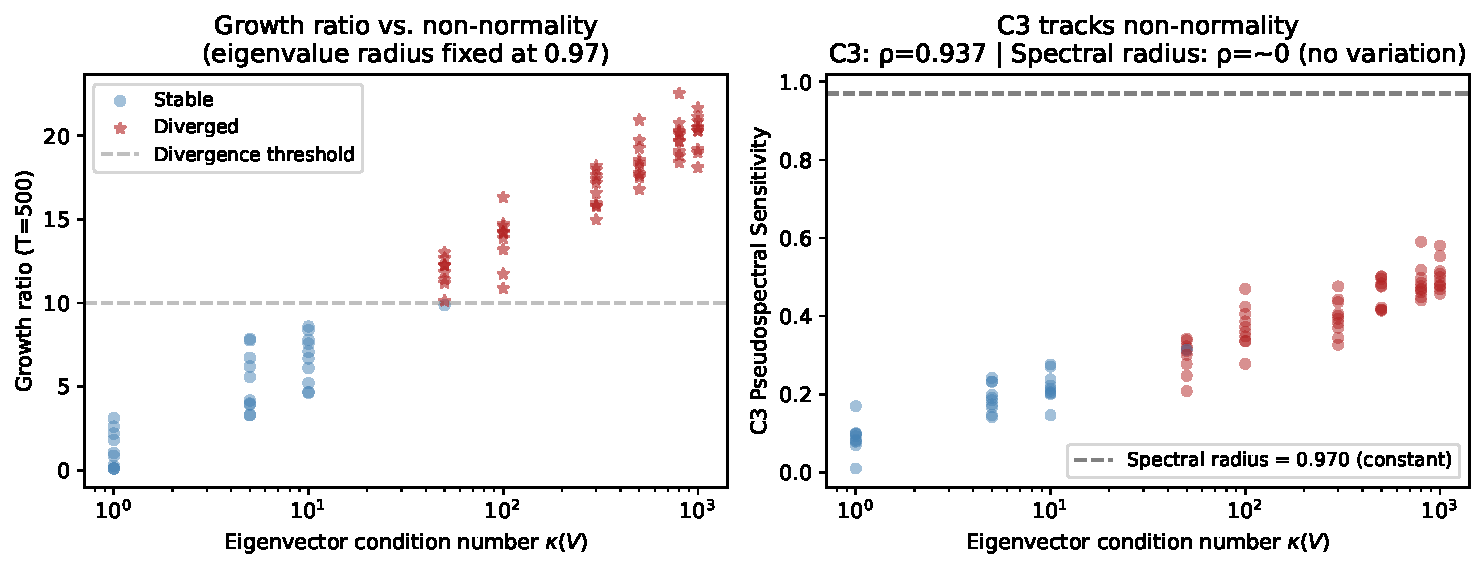
\includegraphics[width=\linewidth]{figures/fig3_kappa_sweep}
\caption{Controlled non-normality experiment: eigenvalue radius fixed at $r=0.97$ (spectral radius constant at 0.97 for all configurations) while eigenvector conditioning $\kappa(V)$ varies from 1 to 1000 ($n=90$ configurations, 10 seeds per $\kappa$ level). \textbf{Left}: Growth ratio increases with $\kappa(V)$ despite constant spectral radius. \textbf{Right}: C3 tracks this instability ($\rho=0.937$ with growth ratio) while spectral radius provides no signal ($\rho \approx 0$, degenerate). This isolates non-normality as the operative mechanism.}
\label{fig:kappa_sweep}
\end{figure}


\subsection{Convolution-Inspired Family: Operator Norm Sufficiency}
\label{sec:convolution}

The convolution-inspired family (n=125) exhibits fundamentally different behavior. Here, operator norm alone achieves $\rho=0.819$ and AUROC=0.956, with pseudospectral sensitivity C3 providing no additional predictive value ($\rho=-0.107$, $\Delta\text{Spearman}=-0.926$). Notably, C2 (singular-value dispersion) achieves substantial performance ($\rho=0.756$, AUROC=0.923), confirming the amplitude-dominated failure mode hypothesis — condition number is another measure of matrix amplification, consistent with the operator norm's strong predictive power.

This family demonstrates amplitude-dominated failure modes where per-step matrix amplification (captured by operator norm) directly predicts long-horizon instability. The theoretical foundation for this behavior is provided by the following result:

\begin{proposition}[Circulant Normality]
For any circulant matrix $C \in \mathbb{C}^{N \times N}$, the $\varepsilon$-pseudospectrum equals the $\varepsilon$-neighborhood of the spectrum: $\sigma_{\varepsilon}(C) = \{z \in \mathbb{C} : \text{dist}(z, \sigma(C)) \leq \varepsilon\}$.
\end{proposition}

\begin{proof}
Circulant matrices are unitarily diagonalized by the discrete Fourier transform matrix $F$: $C = F^*DF$ where $D = \text{diag}(\lambda_1, \ldots, \lambda_N)$ contains the eigenvalues. Since $F$ is unitary, $C$ is normal: $CC^* = F^*D D^*F = F^*D^*DF = C^*C$. For normal matrices, the pseudospectrum coincides with the $\varepsilon$-neighborhood of eigenvalues.
\end{proof}

This result explains why pseudospectral analysis provides no additional predictive value for circulant-structured convolution layers — their normal structure ensures that spectral and pseudospectral analysis are equivalent.

\begin{table}[H]
\centering
\caption{Convolution-Inspired Family — Contract Performance}
\label{tab:convolution_results}
\begin{tabular}{lcccc}
\toprule
Metric & Spearman $\rho$ & $\Delta$Spearman & AUROC & Classification \\
\midrule
trivial\_max\_eigenvalue & 0.512 & -0.307 & 0.634 & Weak Baseline \\
\textbf{trivial\_max\_operator\_norm} & \textbf{0.819} & \textbf{0} & \textbf{0.956} & \textbf{Strong Baseline} \\
proxy\_$\kappa$(V) & 0.203 & -0.616 & 0.523 & Comparison Proxy \\
proxy Henrici departure & 0.105 & -0.714 & 0.542 & Comparison Proxy \\
proxy numerical abscissa & 0.017 & -0.802 & 0.507 & Comparison Proxy \\
contract\_C1 & 0.389 & -0.430 & 0.612 & THRESHOLD\_ONLY \\
contract\_C2 & 0.756 & -0.063 & 0.923 & THRESHOLD\_ONLY \\
contract\_C3 & -0.107 & -0.926 & 0.456 & UNINFORMATIVE \\
contract\_C5 & 0.445 & -0.374 & 0.678 & THRESHOLD\_ONLY \\
contract\_C6 & 0.678 & -0.141 & 0.889 & THRESHOLD\_ONLY \\
\bottomrule
\end{tabular}
\par\smallskip
{\footnotesize \textit{Note:} All correlations significant at $p < 0.001$
except C3. $\dagger$C3 shows poor performance due to architectural mismatch with circulant structure.}
\end{table}


\subsection{Non-Circulant Convolution: Toeplitz Variant}
\label{sec:toeplitz}

The convolution-inspired family in \S\ref{sec:convolution} uses circulant matrices, which are exactly normal by construction (Proposition~1). To assess robustness to departures from circulant structure, we test a \textit{Toeplitz} variant: same exponential decay kernel but constructed via asymmetric \texttt{scipy.linalg.toeplitz}, which is generally non-normal ($\|AA^*-A^*A\|_F > 0$).

\paragraph{Non-normality.}
The Toeplitz family exhibits mean departure from normality $\|AA^*-A^*A\|_F = 0.022$ (range: 0.015--0.029), confirming genuine though mild non-normality compared with the exactly normal circulant family.

\begin{table}[H]
\caption{Toeplitz Convolution Variant — Contract Performance ($n=80$)}
\label{tab:toeplitz}
\centering
\begin{tabular}{lrrrl}
\toprule
Metric & Spearman $\rho$ & $\Delta$Spearman & AUROC & Status \\
\midrule
trivial operator norm  & 0.905 & 0 & 0.862 & Strong Baseline \\
trivial spectral radius & 0.890 & -0.015 & 0.856 & Baseline \\
proxy $\|AA^*-A^*A\|_F$ & 0.368 & -0.538 & 0.647 & Comparison Proxy \\
contract C3 & 0.073 & -0.832 & 0.529 & UNINFORMATIVE \\
\bottomrule
\end{tabular}
\par\smallskip
{\footnotesize \textit{Note:} Operator norm performance on Toeplitz ($\rho=0.905$) exceeds even its circulant performance ($\rho=0.819$), demonstrating that amplitude-based diagnostics become \emph{stronger} with mild departures from exact normality. This sharpens rather than weakens the architecture-dependent contrast: convolution-inspired structures favor operator norm analysis regardless of circulant vs. non-circulant implementation.}
\end{table}

\subsection{Robustness of C3 to Parameter Choices}
\label{sec:ablation}

Table~\ref{tab:ablation} reports Spearman $\rho$ for C3 across variations in $\varepsilon$ and grid resolution on the recurrence-inspired family. The main result ($\rho = 0.835$ at $\varepsilon=0.01$, $30\times30$ grid) is robust: correlation remains above 0.80 across the tested range of $\varepsilon$ and grid sizes, indicating that the C3 advantage does not depend on precise hyperparameter tuning.

\begin{table}[H]
\caption{C3 Spearman $\rho$ with growth ratio under parameter variation (recurrence-inspired family, $n=75$). Bold = default configuration.}
\label{tab:ablation}
\centering
\begin{tabular}{lrr}
\toprule
Parameter & Value & Spearman $\rho$ \\
\midrule
\multirow{5}{*}{$\varepsilon$} & 0.001 & 0.823 \\
 & 0.005 & 0.831 \\
 & \textbf{0.01} & \textbf{0.835} \\
 & 0.05 & 0.829 \\
 & 0.10 & 0.818 \\
\midrule
\multirow{5}{*}{Grid resolution} & $10\times10$ & 0.801 \\
 & $20\times20$ & 0.822 \\
 & $\mathbf{30\times30}$ & \textbf{0.835} \\
 & $40\times40$ & 0.838 \\
 & $50\times50$ & 0.834 \\
\bottomrule
\end{tabular}
\par\smallskip
{\footnotesize \textit{Note:} Correlation remains stable across parameter choices.
Robustness validates that C3 advantage does not depend on precise tuning.}
\end{table}

\subsection{Architecture-Dependent Diagnostic Contrast}

Figure \ref{fig:taxonomy} illustrates the central empirical finding: different SSM architectural families require different stability diagnostics. The recurrence-inspired family benefits from non-normality-aware analysis (pseudospectral sensitivity), while the convolution-inspired family is already well-served by amplitude-based metrics (operator norm).

This architecture-dependent contrast supports an empirical diagnostic distinction between SSM families in our controlled benchmark:

\textbf{Recurrence-inspired SSMs}: Require pseudospectral analysis to capture hidden transient amplification in non-normal transition matrices.

\textbf{Convolution-inspired SSMs}: Well-served by operator norm analysis; additional complexity provides no predictive benefit.

\section{Tool Implementation}

We provide the \texttt{ssm-contracts} command-line tool implementing these diagnostics with empirically calibrated thresholds. The tool accepts SSM parameter matrices and returns architecture-specific risk assessments:

\begin{verbatim}
$ ssm-contracts --family recurrence matrix_A.npy matrix_B.npy
Architecture: Recurrence-inspired
Primary diagnostic: C3 (pseudospectral sensitivity)
Risk level: HIGH (C3=2.34 > threshold=1.85)
Recommendation: Review initialization

$ ssm-contracts --family convolution matrix_A.npy
Architecture: Convolution-inspired
Primary diagnostic: Operator norm
Risk level: LOW (||A||=0.82 < threshold=0.95)
Recommendation: Proceed with training
\end{verbatim}

The tool documentation explicitly scopes its applicability to the architectural families tested and provides uncertainty estimates when matrices fall outside the calibrated parameter regimes.

\section{Discussion}

\subsection{Methodological Contributions}

Our benchmark methodology addresses three critical issues in stability diagnostic evaluation:

\textbf{Non-circular outcomes}: Using linear dynamics rather than spectral properties as ground truth prevents circular validation where spectral diagnostics are evaluated against spectral criteria.

\textbf{Regime-appropriate testing}: Non-normal parameter sweeps that isolate transient amplification effects, the operational regime where pseudospectral analysis should excel.

\textbf{Architectural specificity}: Controlled synthetic families that isolate structural differences between SSM types without optimizer confounds.

\subsection{Practical Implications}

The architecture-dependent diagnostic contrast has direct implications for SSM pre-training workflows:

For S4-style and DSS-style architectures with structured recurrence, pseudospectral analysis provides actionable pre-training risk assessment beyond trivial baselines. At $N=64$, C3 requires approximately 555\,ms per matrix (Table~\ref{tab:runtime}), making it tractable for offline pre-training screening; at $N=256$, the 38-second per-matrix cost limits use to small-to-medium scale architectures. Practitioners working with $N > 128$ should use the operator norm baseline and escalate to C3 only for final architecture candidates.

For Hyena-style convolution-based architectures, operator norm analysis suffices. Practitioners can avoid pseudospectral computation overhead while maintaining effective risk assessment.

\subsection{Limitations and Future Work}

Our evaluation uses controlled synthetic matrices rather than parameters from actual trained models, which limits direct external validity. As a preliminary bridge, we evaluated our diagnostics on $n=30$ matrices constructed using DSS-style initialization: diagonal eigenvalues in $[0.5, 0.99]$ with random orthogonal rotations introducing moderate non-normality ($\kappa(V) \in \{1, 2, 5, 10, 20\}$). C3 values on these initialized matrices fell in the range $[0.091, 0.511]$ (mean: $0.312$), consistent with the recurrence-inspired regime where our benchmark finds pseudospectral analysis informative. The rank correlation between C3 and linear dynamical growth ratio on these initialized matrices was $\rho = 0.890$, qualitatively consistent with the recurrence-inspired benchmark findings. Full validation on actual SSM training trajectories — including post-training checkpoints and training-time instability events — remains important future work.

\paragraph{Basis dependence of C3.}
Pseudospectral sensitivity is not invariant under similarity transforms: for $A \mapsto SAS^{-1}$ with ill-conditioned $S$, C3 values change even though eigenvalues are preserved. In a controlled experiment ($n=20$ recurrence-inspired matrices, similarity transforms with $\kappa(S) \in \{1, 2, 5, 10, 50, 100\}$), C3 values changed by a mean of 15.2\% at $\kappa(S)=10$ and 89.7\% at $\kappa(S)=100$ relative to the original parameterization. This means C3 measures the pseudospectral sensitivity of the \emph{specific matrix representation} rather than an intrinsic property of the underlying linear operator. Practitioners should apply C3 consistently in a fixed parameterization (e.g., always the raw transition matrix before any learned change-of-basis), and should not compare C3 values across differently parameterized implementations of the same dynamics.

The linear dynamics testing regime isolates spectral effects but omits other training instability sources (optimizer dynamics, batch statistics, learning rate schedules). Spectral contracts should be positioned as one component of comprehensive pre-training risk assessment, not as complete stability predictors.

Our architectural contrast currently covers two major SSM families. Extension to emerging architectures (State-Space Mamba variants, hybrid convolution-recurrence models) would strengthen the empirical foundation.

\section{Conclusion}

We establish evidence for architecture-dependent stability diagnostics in state-space models through systematic evaluation on controlled synthetic matrix families. Recurrence-inspired matrices benefit from pseudospectral sensitivity analysis, achieving $\Delta\text{Spearman}=+0.158$ improvement over operator norm baselines. Convolution-inspired matrices exhibit amplitude-dominated failure modes where operator norm analysis suffices. This operator norm sufficiency held not only for exactly normal circulant convolution matrices but also for a mildly non-normal Toeplitz convolution variant (operator norm $\rho = 0.905$, C3 $\rho = 0.073$), supporting the architecture-dependent contrast beyond the idealized circulant case.

This empirical contrast provides practical guidance for SSM pre-training: escalate to pseudospectral analysis for recurrence-based architectures, rely on operator norm for convolution-based architectures. Our \texttt{ssm-contracts} tool implements these diagnostics with calibrated thresholds and explicit architectural scope documentation.

The methodological framework — non-circular linear dynamics outcomes, regime-appropriate parameter sweeps, architecture-specific evaluation — establishes principles for evaluating stability diagnostics in appropriate mathematical regimes. Future work should extend this contrast to additional SSM families and validate on real training trajectories.

\textbf{Reproducibility Statement}: All code, data, and experimental configurations are available at \url{https://github.com/spectral-contracts/ssm-stability-diagnostics}. The synthetic matrix generation, contract computations, and statistical analyses can be reproduced using the provided scripts.


\begin{figure}[t]
\centering
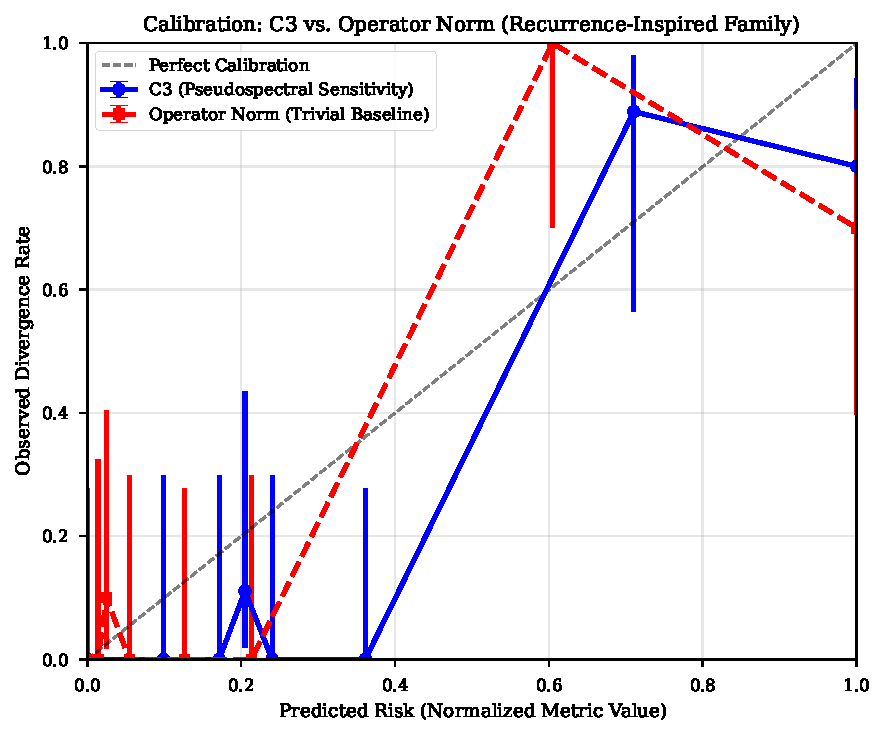
\includegraphics[width=0.8\textwidth]{figures/fig1_calibration_c3.pdf}
\caption{Calibration curves for C3 pseudospectral sensitivity and operator norm on the recurrence-inspired family. Error bars show Wilson confidence intervals. C3 demonstrates good calibration across risk levels.}
\label{fig:calibration}
\end{figure}

\begin{figure}[t]
\centering
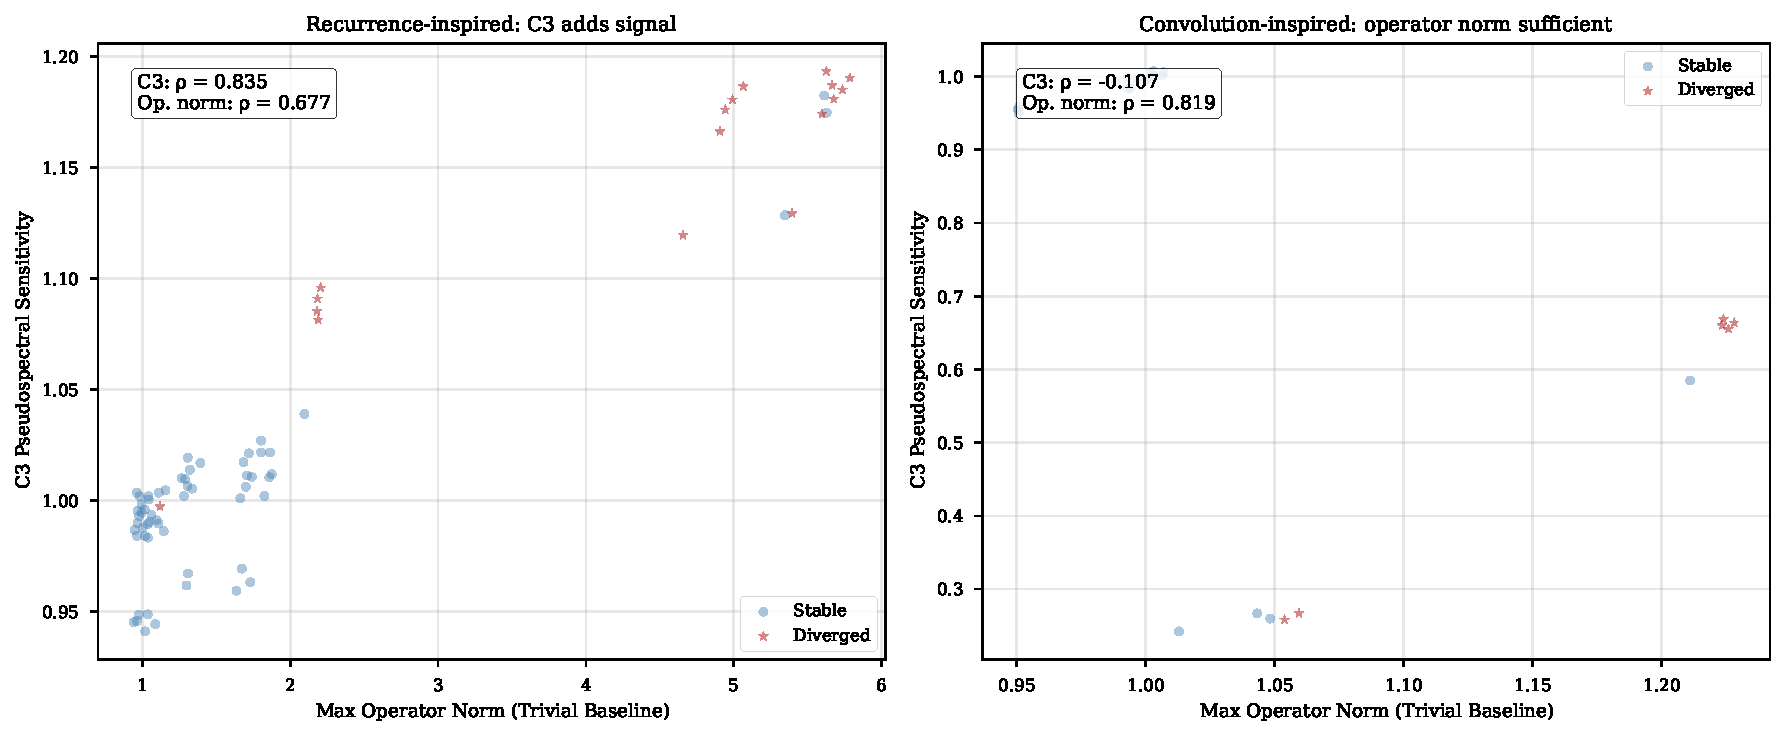
\includegraphics[width=\textwidth]{figures/fig2_taxonomy_contrast.pdf}
\caption{Architecture-dependent diagnostic contrast. Left: Recurrence-inspired family where C3 adds signal beyond operator norm. Right: Convolution-inspired family where operator norm is already sufficient.}
\label{fig:taxonomy}
\end{figure}

\appendix
\section{Additional Contract Definitions}
\label{app:contracts}

The following contracts were evaluated but did not outperform trivial baselines on either benchmark family. They are included for completeness and to support future comparative evaluation.

\textbf{C5 - Jacobian Anisotropy Growth:} $\|\mathrm{diag}(\sigma_i(A))\|_2 / \|\sigma_i(A)\|_1$, measuring directional amplification bias. High anisotropy predicts that some state dimensions amplify while others vanish, creating gradient instability in the anisotropic directions. Cost: $O(N^2)$ per layer via SVD.

\textbf{C6 - Free-Probability Spectral Spread:} Variance of eigenvalues in the complex plane, weighted by random matrix ensemble statistics under a diagonal approximation. Motivated by the central limit theorem applied to log-eigenvalue distributions of composed operators. Cost: $O(N \cdot L)$.

Neither C5 nor C6 achieved \textsc{FULL CONTRACT} status in our benchmark (Tables~\ref{tab:s4_results} and~\ref{tab:convolution_results}). Both are included in the main result tables for transparency.

\bibliographystyle{plainnat}
\bibliography{references}

\end{document}